\chapter{Lezione 18/03/2025}

\subsubsection{Esempio: \textit{il piano in coordinate cartesiani}}

Nel caso del piano, le coordinate cartesiane sono $(x, y)$ e la metrica è data da:

$$
u, v \rightarrow x, y
\quad \Rightarrow \quad
g_{ij} = 
\begin{pmatrix}
    1 & 0 \\
    0 & 1
\end{pmatrix}
$$

$$
ds^2 = g_{ij} du^i du^j = \sum_{ij} g_{ij}du^udu^j = du^2 + dv^2
$$


\subsubsection{Esempio: \textit{il piano in coordinate polari}}

Nel caso del piano in coordinate polari, le coordinate sono $(r, \theta)$ e la metrica è data da:

$$
ds^2 = dr^2 + r^2 d\theta^2,
\quad 
\quad 
g_{ij} = \begin{pmatrix}
    1 & 0 \\
    0 & r^2
\end{pmatrix},
\quad
\quad
g^{ij} = \begin{pmatrix}
    1 & 0 \\
    0 & \dfrac{1}{r^2}
\end{pmatrix}.
$$

$$
\dfrac{d^2u^i}{ds^2} + \Gamma_{jk}^i \dfrac{du^j}{ds} \dfrac{du^k}{ds} = 0
$$

$
\Gamma_{jk}^i = \dfrac{1}{2} g^{ir} \left( \dfrac{\partial g_{jr}}{\partial u^k} + \dfrac{\partial g_{kr}}{\partial u^j} - \dfrac{\partial g_{jk}}{\partial u^r} \right) \quad \text{ricordiamo la simmetria su $j$ e $k$}
$

\begin{itemize}

\item Se $i = r = 1$:

$$
\Gamma_{jk}^1 = \dfrac{1}{2} g^{11} \left( \dfrac{\partial g_{j1}}{\partial u^k} + \dfrac{\partial g_{k1}}{\partial u^j} - \dfrac{\partial g_{jk}}{\partial u^1} \right) \quad \text{perchè $g^{12} = 0$}
$$

\item Se $j = k = 2$:

$$
\Gamma_{22}^1 = \dfrac{1}{2} g^{11} \left( - \dfrac{\partial g_{22}}{\partial u^1} \right) = - \dfrac{1}{2} g^{11} \dfrac {\partial g_{22}}{\partial r} = - \dfrac{1}{2} \cdot 1 \cdot \dfrac{\partial r^2}{\partial r} = - r
$$

\item Se $i = r = 2$:

$$
\Gamma_{jk}^2 = \dfrac{1}{2} g^{22} \left( \dfrac{\partial g_{j2}}{\partial u^k} + \dfrac{\partial g_{k2}}{\partial u^j} - \dfrac{\partial g_{jk}}{\partial u^2} \right) \quad \text{perchè $g^{21} = 0$}
$$

\item Se $j = 1, k = 2$:

$$
\Gamma_{12}^2 = \dfrac{1}{2} g^{22} \left( \dfrac{\partial g_{12}}{\partial u^2} + \dfrac{\partial g_{22}}{\partial u^1} - \dfrac{\partial g_{12}}{\partial u^2} \right) = \dfrac{1}{2} \cdot \dfrac{1}{r^2} \cdot 0 = 0
$$

\end{itemize}

Si ottiene quindi:

$$
\boxed{\Gamma_{11}^1 = \Gamma_{12}^1 = \Gamma_{11}^2 = \Gamma_{22}^2 = 0}
$$

Otteniamo quindi il sistema:

\begin{alignat}{2}
\tag*{(I)}\quad & \dfrac{d^2 r}{ds^2} - r \left( \dfrac{d\theta}{ds} \right)^2 = 0 \\
\tag*{(II)}\quad & \dfrac{d^2 \theta}{ds^2} + \dfrac{2}{r} \left( \dfrac{dr}{ds} \right) \left( \dfrac{d\theta}{ds} \right) = 0
\end{alignat}

\dots

\newpage

In un intorno infinitesimo di un punto è sempre possibile scegliere un sistema di coordinate in cui la matrice dei componenti metrici
$
\scriptsize
g_{ij} = \begin{pmatrix} 1 & 0 \\ 0 & 1 \end{pmatrix}
$
ed in cui le derivate parziali $g_{ij,k}$ sono nulle. Tale sistema viene definito \emph{localmente euclideo}.

Per capire come ciò sia possibile, ricordiamo che la trasformazione della metrica da $g_{ij}$ a $g'_{kl}$ è:
$$
g'_{kl} = \frac{\partial u^i}{\partial u'^k} \frac{\partial u^j}{\partial u'^l}\, g_{ij}.
$$
Espandiamo $g'_{kl}$ attorno al punto $x_0$:
$$
g'_{kl}(x) = g'_{kl}(x_0) + g'_{kl,m}(x_0)\,(x^m - x^m_0) + \frac{1}{2}\, g'_{kl,mn}(x_0)\,(x^m - x^m_0)(x^n - x^n_0) + \cdots,
$$
dove
$$
g'_{kl}(x_0) = \Biggl[ \frac{\partial u^i}{\partial u'^k} \frac{\partial u^j}{\partial u'^l}\, g_{ij} \Biggr]_{x_0},
$$
$$
g'_{kl,m}(x_0) = \Biggl[ \frac{\partial u^i}{\partial u'^k} \frac{\partial u^j}{\partial u'^l}\, g_{ij,m} \Biggr]_{x_0} 
+ \Biggl[ \frac{\partial^2 u^i}{\partial u'^m \partial u'^k} \frac{\partial u^j}{\partial u'^l}\, g_{ij} \Biggr]_{x_0}
+ \Biggl[ \frac{\partial u^i}{\partial u'^k} \frac{\partial^2 u^j}{\partial u'^m \partial u'^l}\, g_{ij} \Biggr]_{x_0}.
$$
Per la simmetria tra gli indici $i$ e $j$ e tra $k$ e $l$, possiamo riscrivere:
$$
g'_{kl,m}(x_0) = \Biggl[ \frac{\partial u^i}{\partial u'^k} \frac{\partial u^j}{\partial u'^l}\, g_{ij,m} \Biggr]_{x_0} 
+ \Biggl[ 2\, \frac{\partial^2 u^i}{\partial u'^m \partial u'^k} \frac{\partial u^j}{\partial u'^l}\, g_{ij} \Biggr]_{x_0}.
$$
Analogamente, per le derivate seconde si ha:
$$
g'_{kl,mn}(x_0) = \Biggl[ \frac{\partial u^i}{\partial u'^k} \frac{\partial u^j}{\partial u'^l}\, g_{ij,mn} \Biggr]_{x_0}
+ \Biggl[ 2\, \frac{\partial^3 u^i}{\partial u'^m \partial u'^n \partial u'^k} \frac{\partial u^j}{\partial u'^l}\, g_{ij} \Biggr]_{x_0} + \text{ derivate prime, seconde e terze},
$$

Supponendo di voler, tramite un'opportuna trasformazione di coordinate, portare $g'_{kl}$ in una forma voluta in un intorno di $x_0$, dobbiamo specificare nella trasformazione le seguenti quantità:

\begin{center}
\begin{tabular}{ccccc}
\toprule
\textbf{Derivatives} & \textbf{2--D} & \textbf{3--D} & \textbf{4--D} & \textbf{N--D}\\
\midrule
$\displaystyle \Bigl(\tfrac{\partial u^i}{\partial u'^k}\Bigr)_{x_0}$
  & $4$
  & $9$
  & $16$
  & $N^2$\\
\midrule
$\displaystyle \Bigl(\tfrac{\partial^2 u^i}{\partial u'^m \partial u'^k}\Bigr)_{x_0}$
  & $6$
  & $18$
  & $40$
  & $\displaystyle \tfrac{N^2(N+1)}{2}$\\
\midrule
$\displaystyle \Bigl(\tfrac{\partial^3 u^i}{\partial u'^m \partial u'^n \partial u'^k}\Bigr)_{x_0}$
  & $8$
  & $30$
  & $80$
  & $\displaystyle \tfrac{N^2(N+1)(N+2)}{6}$\\
\bottomrule
\end{tabular}
\end{center}

D'altro canto, il numero dei valori e delle derivate indipendenti del tensore metrico risulta:

\begin{center}
    \begin{tabular}{lcccc}
    \toprule
     & \textbf{2--D} & \textbf{3--D} & \textbf{4--D} & \textbf{N--D}\\
    \midrule
    $\displaystyle g'_{kl}(x_0)$
       & $3$
       & $6$
       & $10$
       & $\displaystyle \frac{N(N+1)}{2}$\\
    \midrule
    $\displaystyle g'_{kl,m}(x_0)$
       & $6$
       & $18$
       & $40$
       & $\displaystyle \frac{N^2(N+1)}{2}$\\
    \midrule
    $\displaystyle g'_{kl,mn}(x_0)$
       & $9$
       & $36$
       & $100$
       & $\displaystyle \Bigl[\tfrac{N(N+1)}{2}\Bigr]^2$\\
    \bottomrule
    \end{tabular}
\end{center}
    

Dalle considerazioni precedenti possiamo trarre le seguenti conclusioni per le dimensioni 2, 3 e 4:

\begin{itemize}
    \item \textbf{2--D:} Se si fissano i valori di $g'_{kl}(x_0)$ si hanno 3 equazioni per 4 coefficienti, lasciando un grado di libertà (la rotazione degli assi attorno a $x_0$). Se si impone $g'_{kl,m}(x_0) \equiv 0$, si dispongono di 6 equazioni per 6 parametri, dunque la condizione è realizzabile. Tuttavia, se si volesse anche annullare $g'_{kl,mn}(x_0)$, si avrebbero 9 equazioni per 8 parametri: il sistema risulta troppo vincolato e non ammette soluzioni, quindi le derivate seconde non possono essere annullate localmente.

    \item \textbf{3--D:} Per fissare $g'_{kl}(x_0)$ ci sono 6 equazioni e 9 parametri, con 3 gradi di libertà associati alla rotazione dello spazio (ad es. gli angoli di Eulero). Si può porre $g'_{kl,m}(x_0) = 0$ (18 equazioni per 18 incognite), ma non $g'_{kl,mn}(x_0) = 0$ (36 equazioni per 30 incognite).

    \item \textbf{4--D (Spazio di Minkowski):} Per imporre $g'_{kl}(x_0)$ si hanno 10 equazioni e 16 parametri, con 6 gradi di libertà (3 rotazioni più 3 trasformazioni di Lorentz). È possibile forzare $g'_{kl,m}(x_0) = 0$ (40 equazioni per 40 incognite), ma non $g'_{kl,mn}(x_0) = 0$ (100 equazioni per 80 incognite).
\end{itemize}

Poiché in un punto si può sempre imporre $g_{ij} = \delta_{ij}$ e $g_{ij,k} = 0$, la curvatura deve necessariamente dipendere dalle derivate seconde di $g_{ij}$. La forma di dipendenza più semplice, plausibilmente, è quella lineare. Prima di indagare se esista un'espressione di questo tipo, occorre affrontare un'altra questione.

\newpage

\section{Derivata Covariante}

Abbiamo visto che la derivata (o gradiente) di un campo scalare $\varphi$, ossia $\frac{\partial \varphi}{\partial u^i}$, è un vettore covariante. Potrebbe sembrare naturale derivare allo stesso modo un campo vettoriale $A_i(u^k)$, ottenendo un tensore di rango due; tuttavia, ciò non avviene. In generale, il differenziale
$$
dA_i \quad\text{(ingrediente essenziale nel rapporto incrementale)}
$$
non si comporta come un tensore. Infatti, dalla legge di trasformazione
$$
A_i \;=\; \frac{\partial u'^k}{\partial u^i}\,A'_k
$$
discende che
$$
dA_i \;=\; \frac{\partial u'^k}{\partial u^i}\,dA'_k
\;+\;
A'_k\,d\!\Bigl(\frac{\partial u'^k}{\partial u^i}\Bigr)
\;=\;
\frac{\partial u'^k}{\partial u^i}\,dA'_k
\;+\;
\frac{\partial^2 u'^k}{\partial u^i\,\partial u^l}\,A'_k\,du^l.
$$
Osserviamo che $dA_i$ è un vettore solo se $\frac{\partial^2 u'^k}{\partial u^i\,\partial u^l} = 0$, ossia se le nuove coordinate $u'^i$ sono funzioni lineari delle $u^i$ (ad esempio, quando si passa da un sistema di coordinate rettilinee a un altro rettilineo).

Perché $dA_i$ non è un vettore? Perché la differenza
$$
dA_i \;=\; A_i(u^i + du^i) \;-\; A_i(u^i)
$$
riguarda due vettori applicati in punti diversi (anche se infinitamente vicini). In un sistema di coordinate generico, i coefficienti di trasformazione variano da punto a punto, quindi tali vettori non si trasformano nello stesso modo. Perché la differenza di due vettori sia a sua volta un tensore, i due vettori devono essere \emph{confrontati nello stesso punto}. Se ambedue si trovano nello stesso punto, allora subiscono la stessa trasformazione, e anche la loro differenza si comporta come un tensore. Ne segue che, per definire una derivata che si comporti da tensore, abbiamo bisogno di una \emph{derivata covariante}.

\begin{figure}[H]
    \centering
    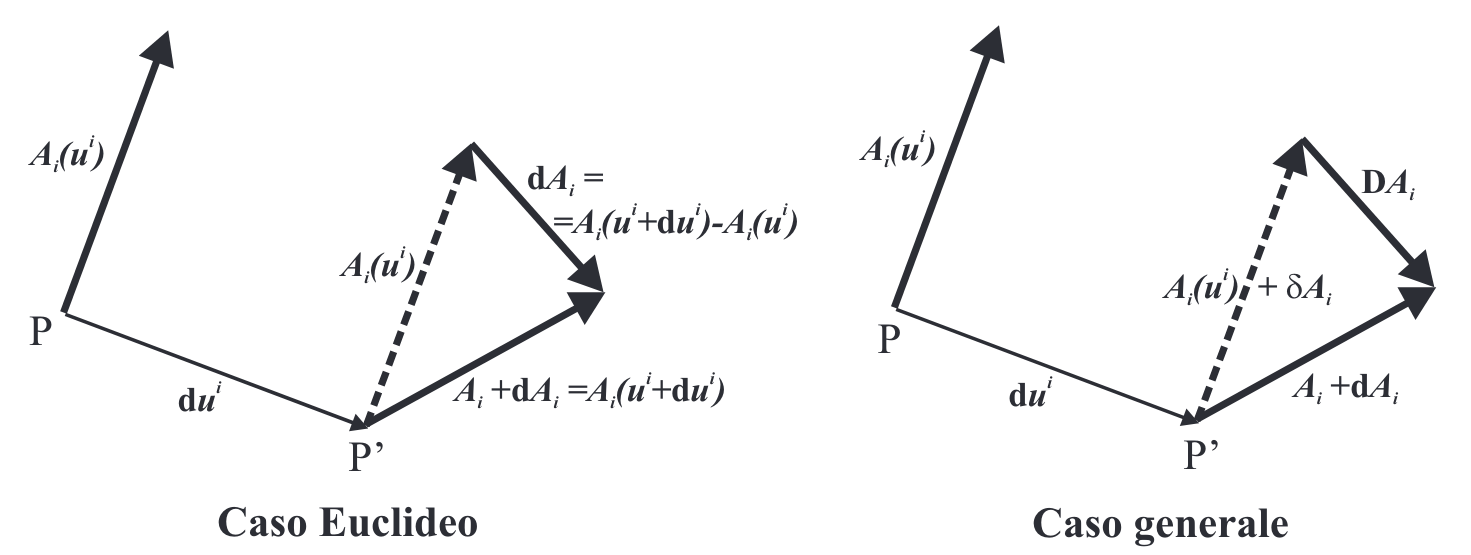
\includegraphics[width=0.7\textwidth]{assets/cov_der.png}
    \caption{Derivata covariante}
    \label{fig:der_cov}
\end{figure}

In uno spazio euclideo, per derivare un vettore $A_i(u^i)$ si procede \emph{spostando parallelamente} $A_i(u^i)$ fino a farne coincidere il punto di applicazione con quello di $A_i(u^i + du^i)$, senza modificarne modulo né direzione. Nel nuovo punto $P'$, si calcola la differenza e si prende il limite del rapporto incrementale:
$$
\lim_{du^i \to 0}\;\frac{A_i(u^i + du^i) \;-\; A_i(u^i)}{du^i}.
$$
Come riprodurre un processo analogo in uno spazio non euclideo? Definiamo il \emph{trasporto parallelo} da $u^i$ a $u^i + du^i$ come quello spostamento che produce una variazione $\delta A_i$ tale che, passando a un sistema localmente euclideo (il che, localmente, è sempre possibile), tale variazione risulti nulla: $\delta A_i = 0$. Pertanto, in $P'$, abbiamo $A_i + dA_i \equiv A_i(u^i + du^i)$ e $A_i + \delta A_i$, corrispondente al trasporto parallelo di $A_i(u^i)$ da $P$ a $P'$. La differenza
$$
DA_i
\;=\;
\bigl(A_i + dA_i\bigr) \;-\; \bigl(A_i + \delta A_i\bigr)
\;=\;
dA_i \;-\;\delta A_i
$$
è un vettore, perché è la differenza di due vettori applicati allo stesso punto. Questo $DA_i$, chiamato \bfit{Diferenziale Assoluto}, ci consente di definire il nuovo tipo di derivata che si comporta come un tensore, la \bfit{derivata covariante}.

\dots
